%%
%% The official i6 slide template _demo_
%% created by Philippe Dreuw and Thomas Deselaers, 2005
%%
%% $Id: slides.tex,v 1.50 2008-07-17 09:21:35 dreuw Exp $
%%
%% Possible options for:
%%  - language       : 'english' (default), 'german'
%%  - page numbering : 'nonumber', 'lastpage' to enable automatic page n/m numbering, 
%%                     'userlastpage' to enable a user defined page n/m numbering using \LastPage command,  
%%                      or leave empty for normal page numbering (default)
%%  - itemize        : 'triangle' or leave empty for bullets (default)
%%  - page layout    : 'vertical' to enable vertical centering on each slide using \vfill ... \vfill (default)
%%                     'demo' to compile images in demo mode, i.e. image files are not necessary 
%%  - encoding       : 'utf-8' to enable utf encoding instead of latin1 (default)
%%  - tools          : 'noblackslide' to disable the black slide at the end which is linked with every slide title, e.g. to write a proof on the blackboard
%%
\documentclass[11pt, a4paper, landscape]{article}
%\usepackage[userlastpage,triangle,demo]{NeyDreuwSlides_Oct08}  % if you don't have the images
\usepackage[userlastpage,triangle,utf-8]{NeyDreuwSlides_Oct08}  % if you don't have the images
\usepackage{snapshot} 
\usepackage{float}

% slides tunning
%\setlength{\footskip}{0pt}       % default ist +30pt - negative Werte nicht moeglich
%\setlength{\headsep}{-10pt}      % default ist +25pt - negative Werte moeglich
%\addtolength{\topmargin}{-5mm}   % bewegt den gesamten Inhalt der Seite nach oben
%\setlength{\textheight}{170mm}   % wenn moeglich nicht veraendern, beinflusst den Inhalt der Seiten und somit auch die Anzahl der Seiten!



% math operators and symbols %%%%%%%%%%%%%%%%%%%%%%%%%%%%%%%%%%%%%%%%%%%%%%%%%%%
\newcommand*{\nat}{\ensuremath{\rm I\!N}\xspace}
\newcommand*{\rel}{\ensuremath{\rm I\!R}\xspace}
\newcommand*{\argmin}{\ensuremath{\operatornamewithlimits{argmin}}\xspace}
\newcommand*{\argmax}{\ensuremath{\operatornamewithlimits{argmax}}\xspace}
\newcommand*{\congmod}{\ensuremath{\operatornamewithlimits{\cong}}\xspace}
\newcommand*{\invers}{\ensuremath{\frac{1}}\xspace}
\newcommand*{\ra}{\ensuremath{\Rightarrow}\xspace}


%%%%%%%%%%%%%%%%%%%%%%%%%%%%%%%%%%%%%%%%%%%%%%%%%%%%%%%%%%%%%%%%%%%%%%%%%%%%%%%%
%% flyspell can read the local ispelldict variable to automatically change the dictionary, 
%% e.g. german-new8, american, english, british, ...
%% 
%% Local IspellDict: american
%% 


%%%%%%%%%%%%%%%%%%%%%%%%%%%%%%%%%%%%%%%%%%%%%%%%%%%%%%%%%%%%%%%%%%%%%%%%%%%%%%%%
% custom packages
\usepackage{fancyvrb} %%% fancy verbatim to enable coloring within verbatim environments
%\usepackage{pst-node} 
%\usepackage[encapsulated]{CJK}
%\newcommand{\cjs}[1]{\begin{CJK}{UTF8}{gbsn}#1\end{CJK}}
%\usepackage{CJK}
%\usepackage{arabtex}
%\novocalize


%%%%%%%%%%%%%%%%%%%%%%%%%%%%%%%%%%%%%%%%%%%%%%%%%%%%%%%%%%%%%%%%%%%%%%%%%%%%%%%%
% Some example hacks work only in combination with the 'pdflatex -shell-escape'
% mode. Try 'make hacks'


%%%%%%%%%%%%%%%%%%%%%%%%%%%%%%%%%%%%%%%%%%%%%%%%%%%%%%%%%%%%%%%%%%%%%%%%%%%%%%%%
\renewcommand*{\title}{Character-based Embeddings of Words with Recurrent Nets}        % main title of the work (used for \TitlePage)
\renewcommand*{\titleshort}{Seminar Template}                                 % short title (used for \lfoot)
\renewcommand*{\occasion}{Seminar Selected Topics in Human Language Technology and Pattern Recognition}%     % (used for \TitlePage) 
\renewcommand*{\occasionshort}{MedBV16 -- Human Language Technology}               % short occasion title (used for \rfoot)
%\renewcommand*{\date}{11. April 2005}                                        % default is \today (used for \TitlePage and \rfoot)
\renewcommand*{\author}{Simon Gr\"atzer}         % all the authors of the work, can be long (used for \TitlePage)
\renewcommand*{\authorshort}{S. Gr\"atzer}                            % all the authors of the work, should be short (used for \lfoot)
%\renewcommand*{\email}{\url{{deselaers,dreuw}@i6.informatik.rwth-aachen.de}}  % all email address(es) of the authors (used for \TitlePage)
\renewcommand*{\mainauthor}{Simon Grätzer}                                   % the author(s) who presented the work (used for \TitlePage)
\renewcommand*{\mainauthoremail}{\url{simon.graetzer@rwth-aachen.de}}    % presenter mail address(es) (used for \FinalPage)
\renewcommand*{\www}{http://www-i6.informatik.rwth-aachen.de/}                % web address (used for \TitlePage _and_ \FinalPage)
\newcommand*{\keywords}{Word Embeddings, LSTM, Language Modeling}                               % keywords, can be used for PDF summary

% will be set into the PDF document summary
\hypersetup{
  pdftitle={\title}, 
  pdfsubject={\occasion},  
  pdfauthor={\author}, 
  pdfkeywords={\keywords},
  % enable automatic page transitions: for endless loop edit in
  % acrobat reader -> preferences -> full screen -> after every X
  % seconds and after last page
  pdfpageduration = 2, 
%  pdfpagetransition = {Glitter /Di 315 /D 5}  
  pdfpagetransition = {Box /M /O /D 1},
}

%%%%%%%%%%%%%%%%%%%%%%%%%%%%%%%%%%%%%%%%%%%%%%%%%%%%%%%%%%%%%%%%%%%%%%%%%%%%%%%%
\listfiles
%%%%%%%%%%%%%%%%%%%%%%%%%%%%%%%%%%%%%%%%%%%%%%%%%%%%%%%%%%%%%%%%%%%%%%%%%%%%%%%%
\begin{document}
%%%%%%%%%%%%%%%%%%%%%%%%%%%%%%%%%%%%%%%%%%%%%%%%%%%%%%%%%%%%%%%%%%%%%%%%%%%%%%%%
\TitlePage

%%%%%%%%%%%%%%%%%%%%%%%%%%%%%%%%%%%%%%%%%%%%%%%%%%%%%%%%%%%%%%%%%%%%%%%%%%%%%%%%
\NewPage\headline{Outline}
\small
\vfill
\begin{enumerate}
\item \hyperlink{sli:introduction}{Introduction}
\item \hyperlink{sli:word-embeddings}{Word Embeddings}
\item \hyperlink{sli:simple}{Generating Word Embeddings}
%\item[] \hyperlink{sli:bibliography}{Bibliography}
%\item[] \hyperlink{sli:appendix}{Appendix}
\end{enumerate}
\vfill
\normalsize
\vfill

%%%%%%%%%%%%%%%%%%%%%%%%%%%%%%%%%%%%%%%%%%%%%%%%%%%%%%%%%%%%%%%%%%%%%%%%%%%%%%%%
\NewPage\headline{Literature} 
\vfill
\begin{itemize}
\item 
\item \cite{tensorflow:word2vec} The tensorflow doumentation by Google Inc.\
\end{itemize}
\vfill 


%%%%%%%%%%%%%%%%%%%%%%%%%%%%%%%%%%%%%%%%%%%%%%%%%%%%%%%%%%%%%%%%%%%%%%%%%%%%%%%%
\NewPage\headline{Introduction} 
\hypertarget{sli:introduction}{}

\vfill
\begin{itemize}
\item Word embeddings are real valued vector representations for words.
\item In this talk I will present a new idea to generate these representations.
  \begin{itemize}
  \item Using recurrent neural networks (LSTM)
  \item Using individual representations of the characters as inputs.
\end{itemize}
\item The resulting model can be used to improve some taks, 
such as language modeling or part-of-speech tagging
\end{itemize}

\begin{figure}[H]
\begin{center}
  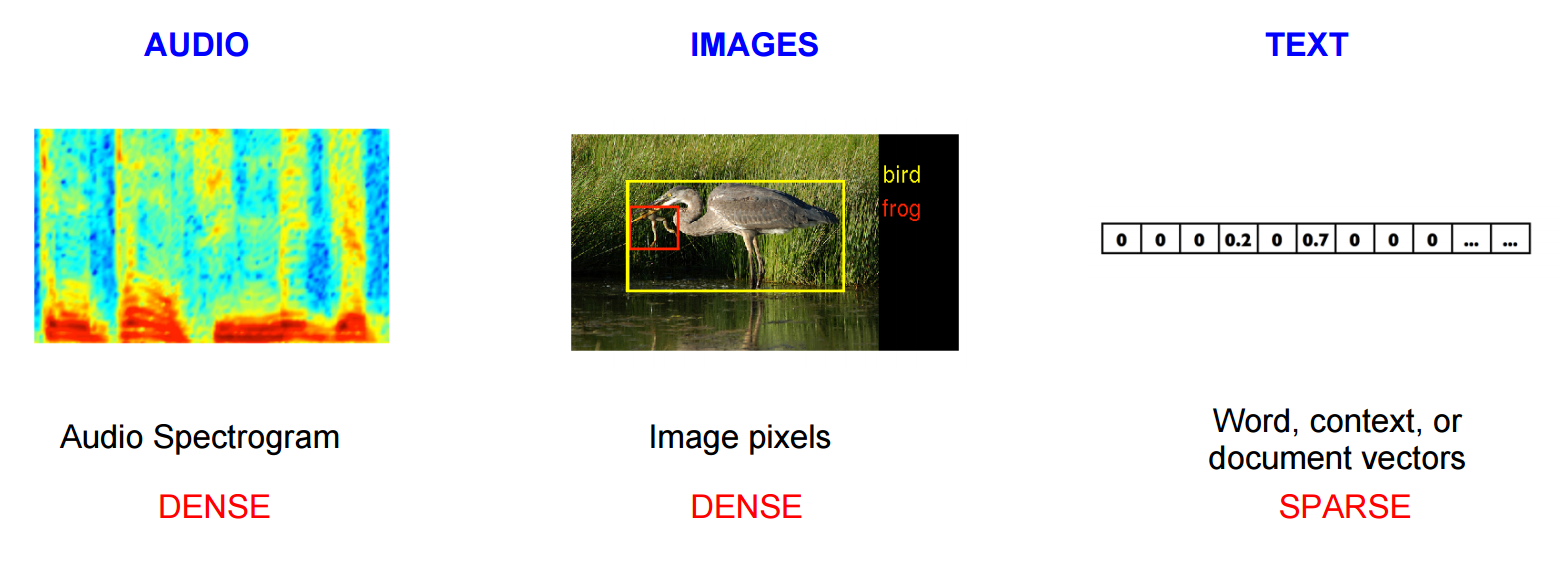
\includegraphics[width=.6\textwidth]{../article/img/audio-image-text}
  \caption{Different input datasets compared to word data~\cite{tensorflow:word2vec}.}
  \label{fig:audio-image-text}
\end{center}
\end{figure}
  The underlying problem is the sparsity of ordinary word representations.
\vfill

%%%%%%%%%%%%%%%%%%%%%%%%%%%%%%%%%%%%%%%%%%%%%%%%%%%%%%%%%%%%%%%%%%%%%%%%%%%%%%%%
\NewPage\headline{Word Embeddings} 
\hypertarget{sli:word-embeddings}{}

\vfill
\begin{figure}[H]
\begin{center}
  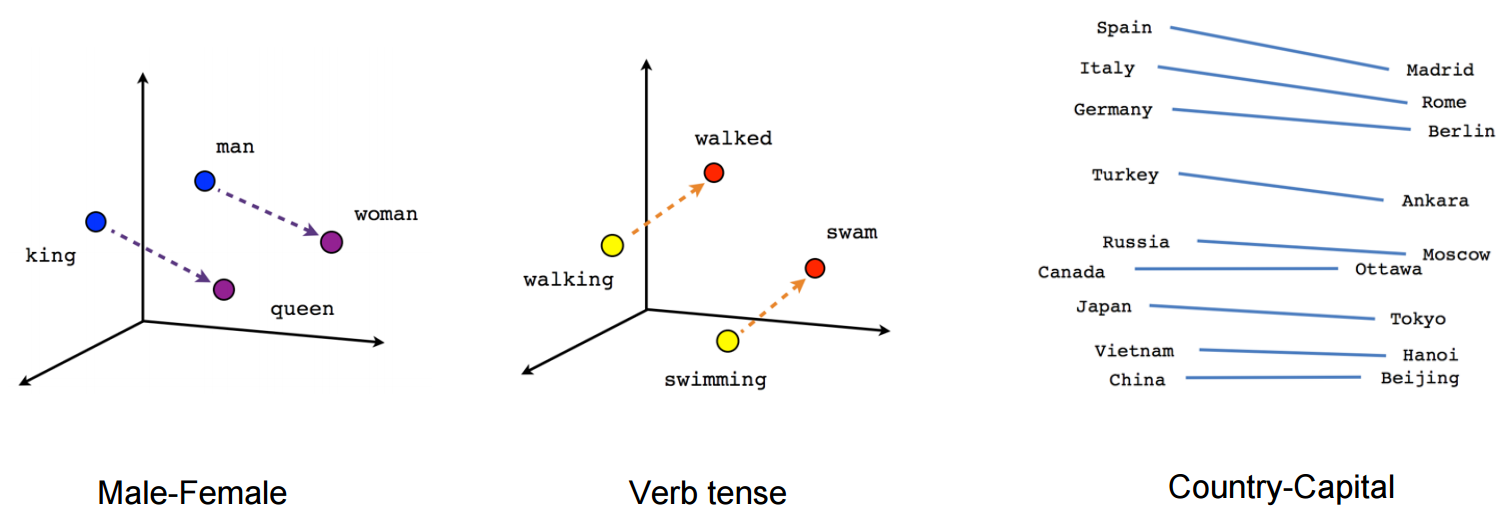
\includegraphics[width=.8\textwidth]{../article/img/linear-relationships}
  \label{fig:linear-relationships}
\end{center}
\end{figure}
\begin{itemize}
\item Words which share semantic meaning tend to occur in the same contexts (Distributional Hypothesis~\cite{Sahlgren2008})
\item A model can learn relationships between words and represent them.
\item Words with a similar meaning should be mapped to nearby points in the same vector space.
\item This captures the intuition that words may be similar along a variety of ways.
\end{itemize}
\vfill

%%%%%%%%%%%%%%%%%%%%%%%%%%%%%%%%%%%%%%%%%%%%%%%%%%%%%%%%%%%%%%%%%%%%%%%%%%%%%%%%
\NewPage\headline{Simple Word Embeddings in a Language Model}
\hypertarget{sli:simple}{}

\vfill
\begin{minipage}[b]{.4\linewidth}
  \begin{center}
    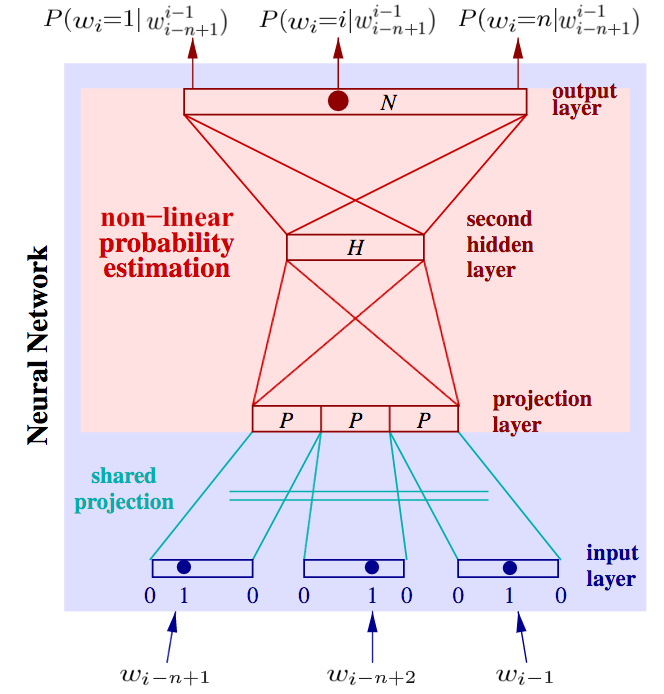
\includegraphics[width=\linewidth]{../article/img/classic_nnlm}
    Classical natural language model
  \end{center}
\end{minipage}
\begin{minipage}[b]{.6\linewidth}
\vfill
\begin{itemize}
\item Language modelling estimates $p(w_1,\dots,w_m) = \prod_{i=1}^{m} p(w_i | w_1,\dots,w_{i-1})$
\item The context is approximated with the previous $n - 1$ words (n-grams)
\item $p(w_1,\dots,w_m) = \prod_{i=1}^{m} p(w_i | w_1,\dots,w_{i-1}) \approx \prod_{i=1}^{m} p(w_i | w_{i-(n-1)},\dots,w_{i-1})$
\end{itemize}
\vfill
\end{minipage}
\vfill

%%%%%%%%%%%%%%%%%%%%%%%%%%%%%%%%%%%%%%%%%%%%%%%%%%%%%%%%%%%%%%%%%%%%%%%%%%%%%%%%
\NewPage\headline{Simple Word Embeddings in a Language Model}

\vfill
\begin{minipage}[b]{.4\linewidth}
  \begin{center}
    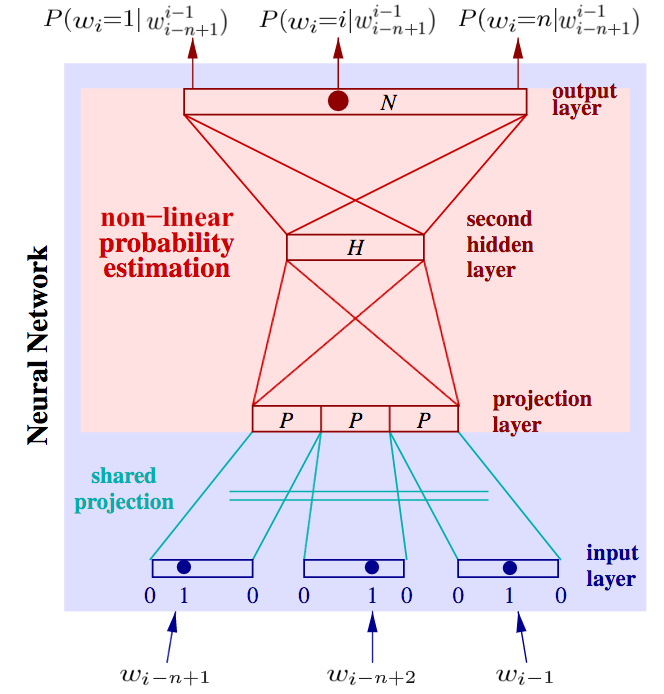
\includegraphics[width=\linewidth]{../article/img/classic_nnlm}
    Classical natural language model
  \end{center}
\end{minipage}
\begin{minipage}[b]{.6\linewidth}
  \begin{itemize}
  \item Word Embeddings are trained end to end, as part of the language model
  \item The word embeddings is essentially the output of the first hidden layer for a word.
  \item The embeddings are stored in a lookup table $P \in \mathbb{R}^{|V| \times d}$. 
      An embeddings is calculated as $e_{w_i}^W = P * 1_{w_i}$
  \end{itemize}
\end{minipage}
\vfill

%%%%%%%%%%%%%%%%%%%%%%%%%%%%%%%%%%%%%%%%%%%%%%%%%%%%%%%%%%%%%%%%%%%%%%%%%%%%%%%%
\NewPage\headline{Repetition: Softmax-Layer}

\vfill
\begin{minipage}[b]{.4\linewidth}
  \begin{center}
    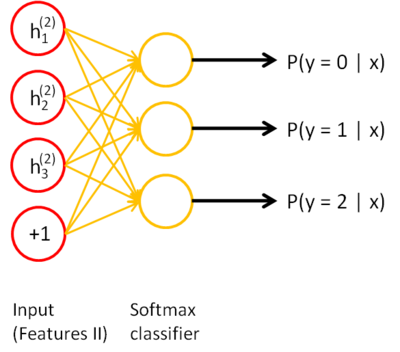
\includegraphics[width=\linewidth]{../article/img/softmax_layer}\\
    $p_k = \sigma(\mathbf{z})_k = \frac{e^{z_k}}{\sum_{k=1}^{|V|} e^{z_k}}$
  \end{center}
\end{minipage}
\begin{minipage}[b]{.6\linewidth}
  \begin{itemize}
  \item The input vector $z$ is computed over the vocabulary: $z_k \forall k \in V$.
  \item The result of the outputs can be interpreted as posterior probabilities.
  \item Probability given the context: $p_k = p(w_i = k | w_{i-n+1}^{i-1})$
  \end{itemize}
\end{minipage}
\vfill

%%%%%%%%%%%%%%%%%%%%%%%%%%%%%%%%%%%%%%%%%%%%%%%%%%%%%%%%%%%%%%%%%%%%%%%%%%%%%%%%
\NewPage\headline{Advanced Word Embeddings: Word2vec}

\vfill
\begin{figure}[H]
\begin{center}
  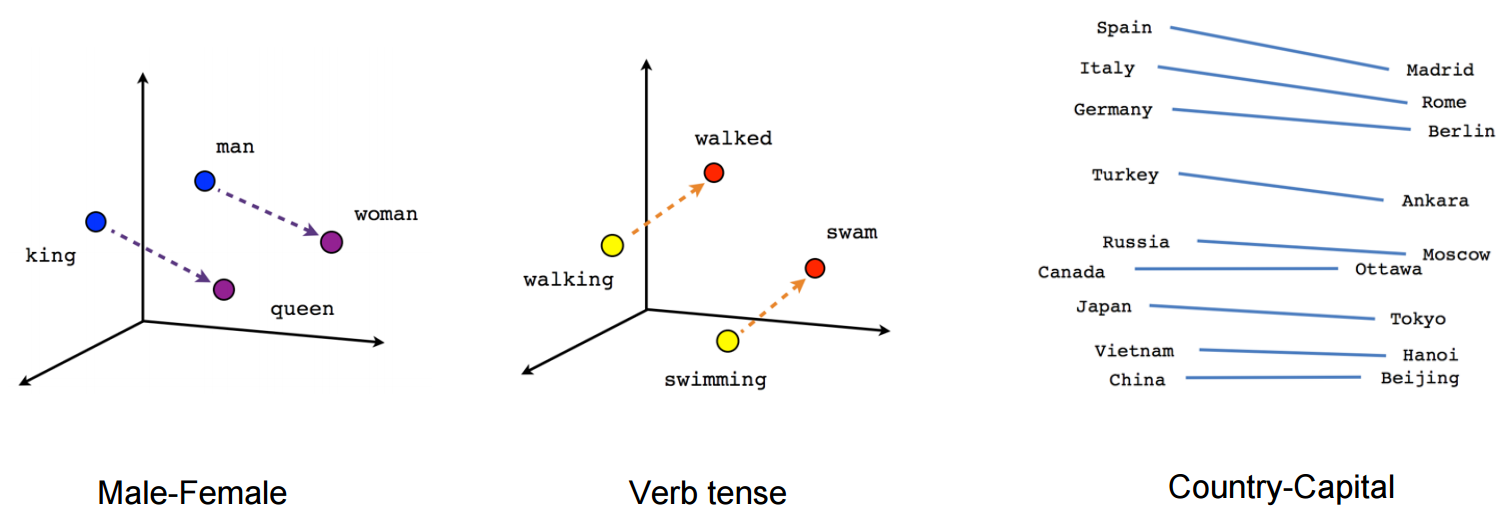
\includegraphics[width=.8\textwidth]{../article/img/linear-relationships}
  \label{fig:classic_nnlm}
\end{center}
\end{figure}
\vfill
\begin{itemize}
\item The Skip-Gram based model from Mikolov et.al.\ was developed at Google.
\item They use n-gram's but invert the model: ${\displaystyle \sum _{-k\leq j-1,\,j\leq k}\log P(w_{t+j}|w_{t})}$
\item ${\displaystyle v(\mathrm {king} )-v(\mathrm {male} )+v(\mathrm {female} )\approx v(\mathrm {queen} )}$
\item Resulting lookup table of embeddings can be reused for other tasks.
\end{itemize}
\vfill

%%%%%%%%%%%%%%%%%%%%%%%%%%%%%%%%%%%%%%%%%%%%%%%%%%%%%%%%%%%%%%%%%%%%%%%%%%%%%%%%
\NewPage\headline{Drawbacks of these Embeddings}

\vfill
\begin{itemize}
\item Each word embedding vector is completly independent. 
\begin{itemize}
  \item The model captures smililar linear correspondences between words embeddings i.e.\
        \textit{cat} and \textit{apple} compared to \textit{cats} and \textit{apples} 
  \item It doesn't capture that the added \textit{s} is responsible for this transformation. 
  \item A word lookup table cannot generate representations for an unknown word.
  \item Even if it's just the plural form of a known word.
\end{itemize}
\item For a large vocabulary it becomes impractical to actually store all word embeddings in a table.
\end{itemize}
\vfill


%%%%%%%%%%%%%%%%%%%%%%%%%%%%%%%%%%%%%%%%%%%%%%%%%%%%%%%%%%%%%%%%%%%%%%%%%%%%%%%%
\NewPage\headline{Reminder: Long-Short Term Memory}

\vfill
\begin{figure}[H]
\begin{center}
  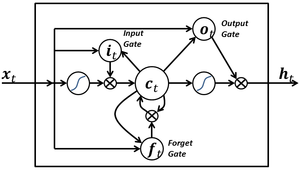
\includegraphics[width=.5\textwidth]{../article/img/Long_Short_Term_Memory}
\end{center}
\end{figure}
\vfill
\begin{itemize}
\item Designed to "remember" inputs over long distances and "forget" them when necessary
\item Works well for time series data
\end{itemize}
\begin{itemize}
\item Gate \(i_t\) to determine when to learn an input value
\item Gate \(f_t\) to determine if it should continue to remember or forget the currently stored value
\item Gate \(o_t\) to determine wether it should output the value.
\item Additionally there are peephole connections and bias values.
\end{itemize}
\vfill


%%%%%%%%%%%%%%%%%%%%%%%%%%%%%%%%%%%%%%%%%%%%%%%%%%%%%%%%%%%%%%%%%%%%%%%%%%%%%%%%
%\NewPage\headline{Repetition: Long-Short Term Memory}
%
%\vfill
%\begin{figure}[H]
%\begin{center}
%  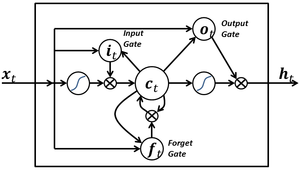
\includegraphics[width=.5\textwidth]{../article/img/Long_Short_Term_Memory}
%\end{center}
%\end{figure}
%\vfill
%Given the input vectors $x_1,\dots,x_m$ a LSTM computes the sequence $h_1,\dots, h_{m+1}$
%\begin{equation}
%\begin{aligned}  
%  i_t &=\sigma(W_{ix} * x_t  + W_{ih} * h_{t-1} + W_{ic} * c_{t-1} + b_i) \\  
%  f_t &=\sigma(W_{fx} * x_t  + W_{fh} * h_{t-1} + W_{fc} * c_{t-1} + b_f) \\
%  o_t &=\sigma(W_{ox} * x_t  + W_{oh} * h_{t-1} + W_{oc} * c_t + b_o) \\  
%  c_t &= f_t \odot c_{t-1} + i_t \odot \tanh(W_{cx} * x_t  + W_{ch} * h_{t-1} + b_c) \\ 
%  h_t &= o_t \odot \tanh(c_t) 
% \end{aligned}
% \end{equation}
% \vfill
% LSTM's avoid the vanishing gradient problem, because
% the activation function in $c_t$ is the identity function.
% \vfill

%%%%%%%%%%%%%%%%%%%%%%%%%%%%%%%%%%%%%%%%%%%%%%%%%%%%%%%%%%%%%%%%%%%%%%%%%%%%%%%%
\NewPage\headline{Character-based Word-Embeddings}

\vfill
\begin{minipage}[b]{.4\linewidth}
  \begin{center}
    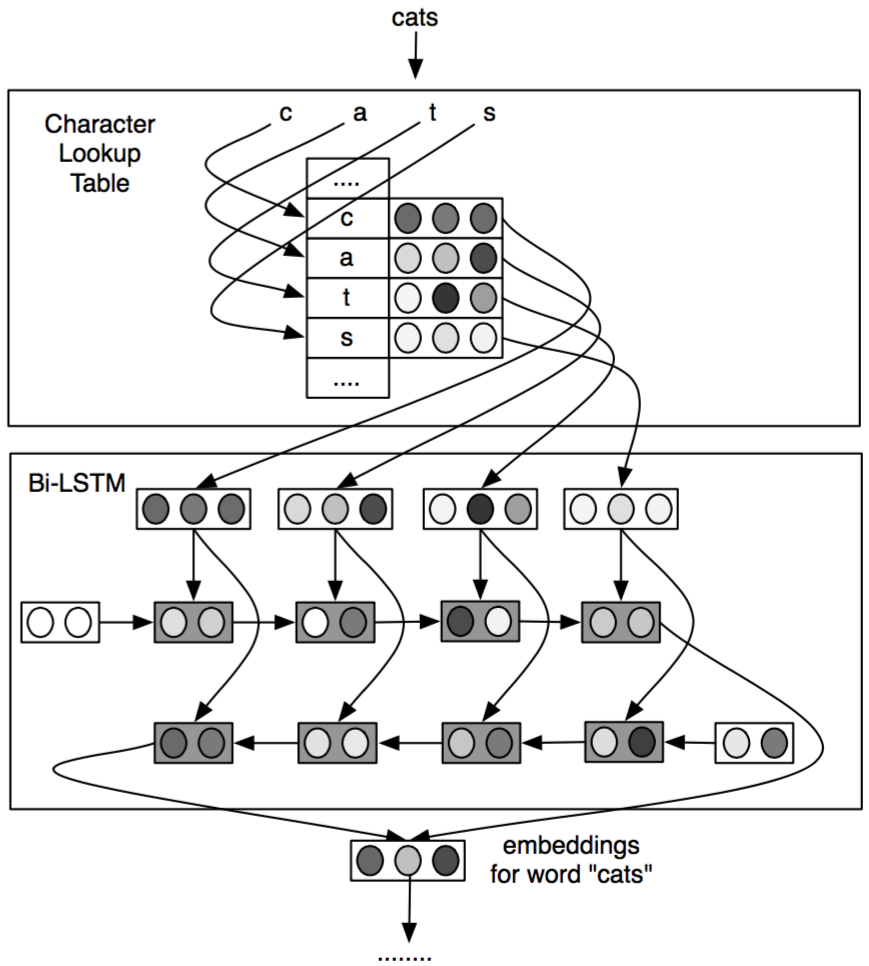
\includegraphics[width=\linewidth]{../article/img/bi-lstm-emeddings}\\
    Character lookup table on top, bidirectional LSTM on the bottom
  \end{center}
\end{minipage}
\begin{minipage}[b]{.6\linewidth}
  Overview:
  \begin{itemize}
  \item Called the "Character to Word" model (C2W)
  \item A word with length $m$ is composed of characters $c_1, \dots, c_m$.
  \item Decompose each word into a sequence of character embeddings $e_{c_1}^C, \dots, e_{c_m}^C$ from the alphabet $C$.
  \item The embeddings are processed and recomposed to form the word-embedding.
  \end{itemize}
\end{minipage}
\vfill

%%%%%%%%%%%%%%%%%%%%%%%%%%%%%%%%%%%%%%%%%%%%%%%%%%%%%%%%%%%%%%%%%%%%%%%%%%%%%%%%
\NewPage\headline{Character-based Word-Embeddings (C2W)}

\vfill
\begin{minipage}[b]{.4\linewidth}
  \begin{center}
    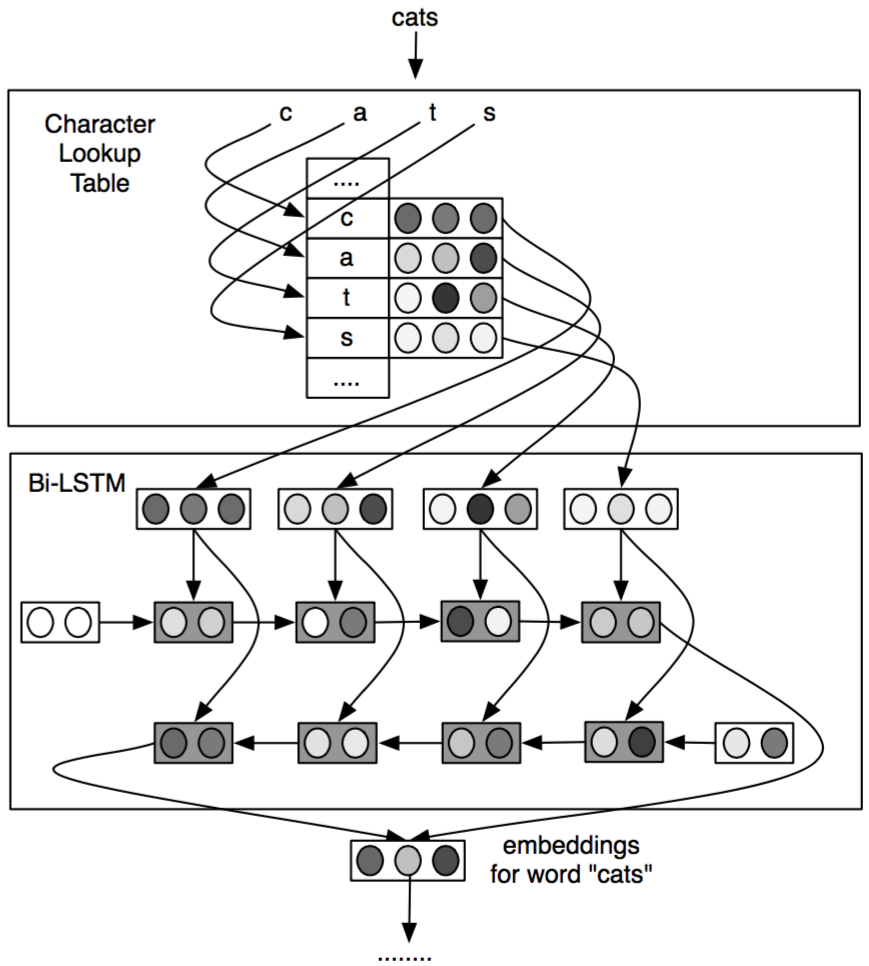
\includegraphics[width=\linewidth]{../article/img/bi-lstm-emeddings}\\
    Character lookup table on top, bidirectional LSTM on the bottom
  \end{center}
\end{minipage}
\begin{minipage}[b]{.6\linewidth}
  Overview:
  \begin{itemize}
  \item A word with length $m$ is composed of characters $c_1, \dots, c_m$.
  \item Decompose each word into a sequence of character embeddings $e_{c_1}^C, \dots, e_{c_m}^C$ from the alphabet $C$.
  \item The embeddings are processed and recomposed to form the word-embedding.
  \end{itemize}
\end{minipage}
\vfill

%%%%%%%%%%%%%%%%%%%%%%%%%%%%%%%%%%%%%%%%%%%%%%%%%%%%%%%%%%%%%%%%%%%%%%%%%%%%%%%%
\NewPage\headline{Character-based Word-Embeddings (C2W)}

\vfill
\begin{minipage}[b]{.4\linewidth}
  \begin{center}
    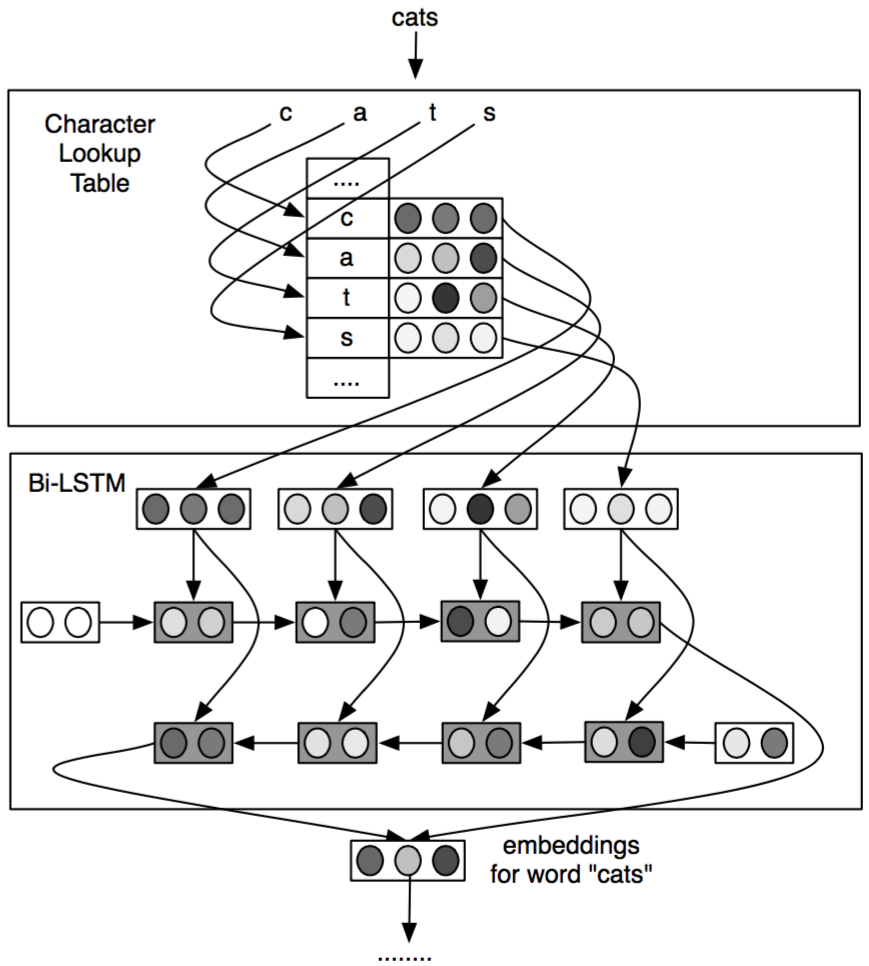
\includegraphics[width=\linewidth]{../article/img/bi-lstm-emeddings}\\
    Character lookup table on top, bidirectional LSTM on the bottom
  \end{center}
\end{minipage}
\begin{minipage}[b]{.6\linewidth}
  Overview:
  \begin{itemize}
  \item A word with length $m$ is composed of characters $c_1, \dots, c_m$.
  \item Decompose each word into a sequence of character embeddings $e_{c_1}^C, \dots, e_{c_m}^C$ from the alphabet $C$.
  \item The sequence is fed to two LSTM units (Bidirectional LSTM), forwards and backwards.
  \item In the end the result is combined by an output layer.
  \end{itemize}
\end{minipage}
\vfill

%%%%%%%%%%%%%%%%%%%%%%%%%%%%%%%%%%%%%%%%%%%%%%%%%%%%%%%%%%%%%%%%%%%%%%%%%%%%%%%%
\NewPage\headline{C2W-Model: Character-Lookup Table}

\vfill
\begin{itemize}
  \item Table of $d_C$ parameters $P_C \in \mathbb{R}^{d_C \times |C|}$ for each character from a predefined character alphabet $C$.
  \item Each Input character is transformed into a $d_C$-dimensional feature vector $e_{c_j}^C$.
  \item We define the projection of characters as $e_{c_j}^C = P_C * 1_{c_j}$.
  \item Similar to the previous projection layer for each word.
\end{itemize}
\vfill

%%%%%%%%%%%%%%%%%%%%%%%%%%%%%%%%%%%%%%%%%%%%%%%%%%%%%%%%%%%%%%%%%%%%%%%%%%%%%%%%
\NewPage\headline{C2W-Model: Bidirectional LSTM Layer}

\vfill
\begin{figure}[H]
\begin{center}
  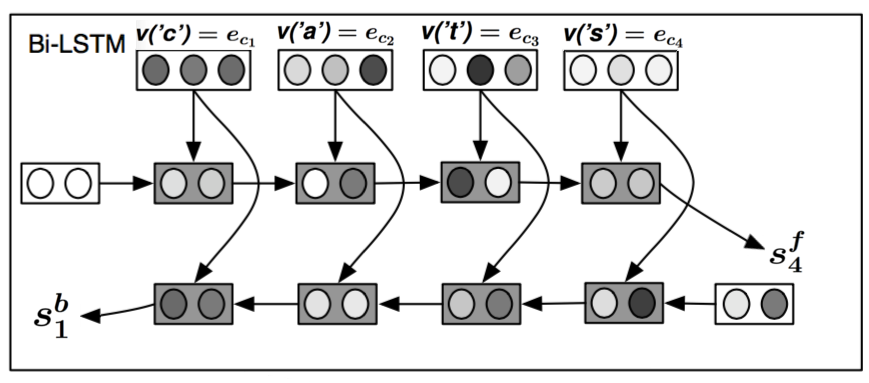
\includegraphics[width=.5\linewidth]{../article/img/brnn-unfolded}
\end{center}
\end{figure}
\begin{itemize}
\item Present every input sequence forwards and backwards to two separate recurrent neural networks 
\item Both RNN's are connected to the same output layer.
\item The network has simultanious access to all inputs before and after the current one.
\item No need for fixed window sizes for the input, the net decides how much context to use.
\item Yields the forward state sequence $s_{0}^f, \dots, s_{m}^f$ and backward state sequence $s_{m}^b, \dots, s_{0}^b$.
\end{itemize}
\vfill


%%%%%%%%%%%%%%%%%%%%%%%%%%%%%%%%%%%%%%%%%%%%%%%%%%%%%%%%%%%%%%%%%%%%%%%%%%%%%%%%
\NewPage\headline{Combining Layer}

\vfill
\begin{itemize}
\item Combines the last states of the forward sequence $s_{m}^f$ and the backwards sequence $s_{0}^b$
\item $e_{w}^C = D^f s_{m}^f + D^b s_{0}^b + b_d$
\item The variables $D^f, D^b, b_d$ are the weights which determine how the states are combined.
\item Automatically learns how much each context is used.
\end{itemize}
\vfill


%%%%%%%%%%%%%%%%%%%%%%%%%%%%%%%%%%%%%%%%%%%%%%%%%%%%%%%%%%%%%%%%%%%%%%%%%%%%%%%%
\NewPage\headline{Character-based Word-Embeddings: Advantages}

\begin{itemize}
\item Simply breaks-up words into simple atomic units.
\item Characters are the simplest atomic unit of words.
\item Aternative: Use Morphemes as atmoic units
  \begin{itemize}
  \item A morpheme is the smallest grammatical unit of a language
  \item e.g.\ "Unbreakable" comprises three morphemes: un-, -break-, and -able.
  \item Would require a morphological analyser
  \end{itemize}
\end{itemize}
\vfill

%%%%%%%%%%%%%%%%%%%%%%%%%%%%%%%%%%%%%%%%%%%%%%%%%%%%%%%%%%%%%%%%%%%%%%%%%%%%%%%%
\NewPage\headline{Applications}

\vfill
We are going to introduce three use cases, where a C2W based model outperforms
other state of the art approches.
\begin{itemize}
\item Language Modelling
\item Part-Of-Speech Tagging
\item Morphological Inflection Generation
\end{itemize}
\vfill


%%%%%%%%%%%%%%%%%%%%%%%%%%%%%%%%%%%%%%%%%%%%%%%%%%%%%%%%%%%%%%%%%%%%%%%%%%%%%%%%
\NewPage\headline{Application 1: Language Modeling}

\vfill
\begin{minipage}[b]{.4\linewidth}
  \begin{center}
    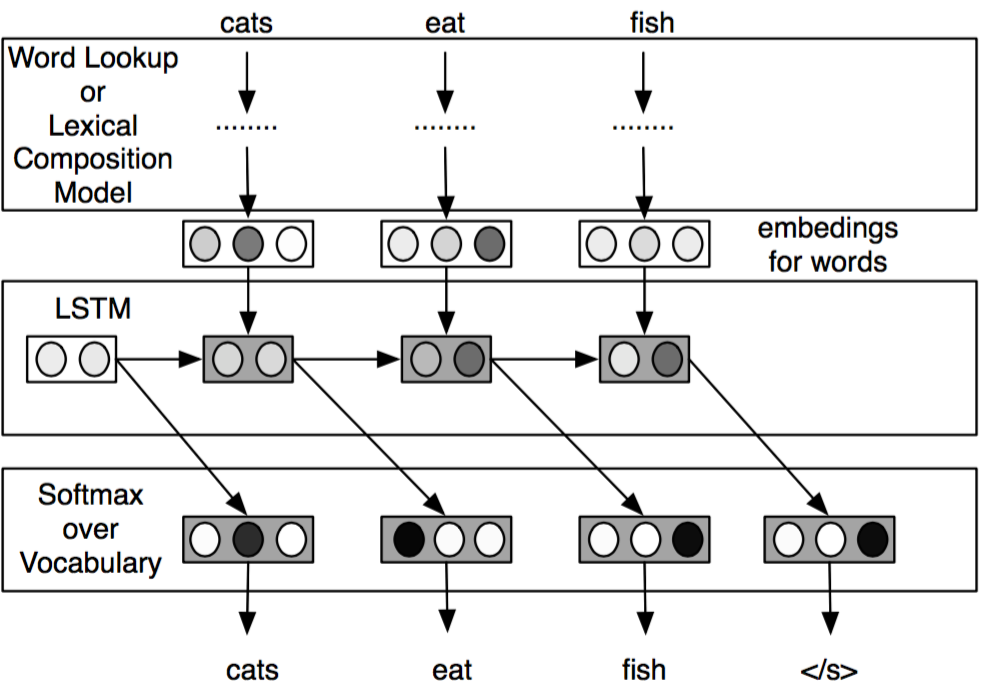
\includegraphics[width=\linewidth]{../article/img/c2w-language-model}
  \end{center}
\end{minipage}
\begin{minipage}[b]{.6\linewidth}
  \begin{itemize}
  \item Uses the word embeddings from the C2W model combined with a LSTM unit.
  \item Every time we input a new word $w_i$ from the sequence the model yields the LSTM state $s_i$.
  \item In the end a softmax layer is used to compute the likelihood $p(w_i = k | w_{i-n+1}^{i-1})$
  \end{itemize}
\end{minipage}
\vfill

%%%%%%%%%%%%%%%%%%%%%%%%%%%%%%%%%%%%%%%%%%%%%%%%%%%%%%%%%%%%%%%%%%%%%%%%%%%%%%%%
\NewPage\headline{Application 1: Evaluation}

\vfill
\begin{itemize}
\item Training is done by
\end{itemize}
\vfill

%%%%%%%%%%%%%%%%%%%%%%%%%%%%%%%%%%%%%%%%%%%%%%%%%%%%%%%%%%%%%%%%%%%%%%%%%%%%%%%%
\NewPage\headline{Application 1: Evaluation}

\vfill
\begin{itemize}
\item TODO include the evalutation tables
\end{itemize}
\vfill

%%%%%%%%%%%%%%%%%%%%%%%%%%%%%%%%%%%%%%%%%%%%%%%%%%%%%%%%%%%%%%%%%%%%%%%%%%%%%%%%
\NewPage\headline{Reminder: Softmax-Layer}

\vfill
\begin{itemize}
\item TODO include the evalutation tables
\end{itemize}
\vfill

%%%%%%%%%%%%%%%%%%%%%%%%%%%%%%%%%%%%%%%%%%%%%%%%%%%%%%%%%%%%%%%%%%%%%%%%%%%%%%%%
% \NewPage\headline{Application 2: Part-Of-Speech Tagging}

%%%%%%%%%%%%%%%%%%%%%%%%%%%%%%%%%%%%%%%%%%%%%%%%%%%%%%%%%%%%%%%%%%%%%%%%%%%%%%%%
% \NewPage\headline{Application 2: Evaluation}


%%%%%%%%%%%%%%%%%%%%%%%%%%%%%%%%%%%%%%%%%%%%%%%%%%%%%%%%%%%%%%%%%%%%%%%%%%%%%%%%
\NewPage\headline{Application 3: Morphological Inflection Generation}

\vfill
\begin{table}
\begin{center}
\begin{tabular}{ l l l l }
  \hline
             & singular & plural \\ \hline
  nominative & Kalb & K\"alber \\
  accusative & Kalb & K\"alber \\
  dative & Kalb & K\"albern \\
  genitive & Kalbes & K\"alber \\
\end{tabular}
\end{center}
\caption{Example of an inflection table for the word "Kalb" }
\end{table}
\vfill
\begin{itemize}
\item Perform morphological transformations, as discussed in Faruqui et al. \cite{DBLP:journals/corr/FaruquiTND15}
\item The transformations are very common in languages like turkish or german.
\item Basic idea is to use a neuronal encoder - decoder architecture.
\item The encoder mirrors the C2W model.
\end{itemize}
\vfill

%%%%%%%%%%%%%%%%%%%%%%%%%%%%%%%%%%%%%%%%%%%%%%%%%%%%%%%%%%%%%%%%%%%%%%%%%%%%%%%%
\NewPage\headline{Application: Morphological Inflection Generation}

\begin{figure}[H]
\begin{center}
  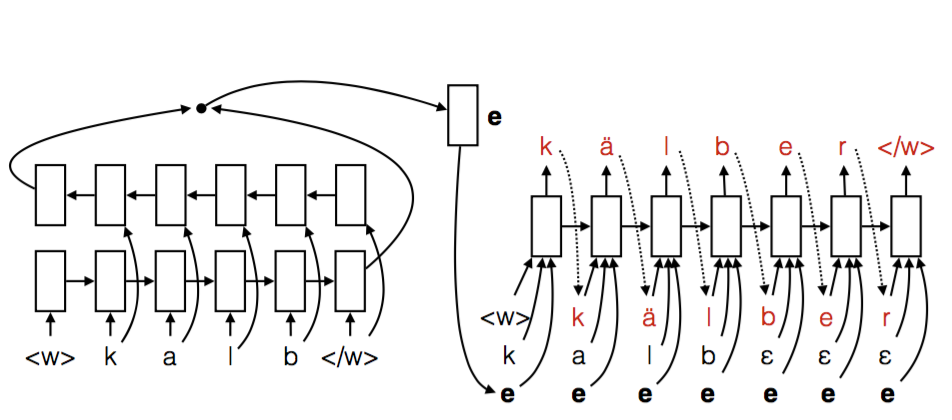
\includegraphics[width=.6\linewidth]{../article/img/inflection-generation}
\end{center}
\end{figure}
\begin{itemize}
\item First: Encoder is virtually identically to C2W model and generates a word embedding $e_{w}$.
\item The decoder is just an LSTM unit which receives the following inputs each timestep:
  \begin{enumerate}
    \item The word embedding $e_{w}$ from the encoder.
    \item Current character of the original word $c_j$
    \item Previous output of the model
  \end{enumerate}
\item Once the input word ends, the  $\epsilon$ character is used instead.
\end{itemize}

%%%%%%%%%%%%%%%%%%%%%%%%%%%%%%%%%%%%%%%%%%%%%%%%%%%%%%%%%%%%%%%%%%%%%%%%%%%%%%%%
\NewPage\headline{Summary}

\vfill
\begin{itemize}
\item Calculating the word embeddings is cheaper than storing them in huge lookup-tables
\item Performance is comparable to other methods
\item Lexical features can be learned automatically
\item Redundancies in lookup-tables are avoided
\item Models scale better with larger vocabularies.
\end{itemize}
\vfill


%%%%%%%%%%%%%%%%%%%%%%%%%%%%%%%%%%%%%%%%%%%%%%%%%%%%%%%%%%%%%%%%%%%%%%%%%%%%%%%%
\NewPage\headline{Backup: Perplexity}

\vfill
\begin{itemize}
\item Measure of how well a probability distribution predicts sample data.
\item Can be interpreted as the number of choices per word position.
\item Defined as $2^{H(p)}=2^{-\sum_x p(x)\log_2 p(x)}$
\item To minimize the perplexity value means to have a better fitting language model.
\end{itemize}
\vfill

\end{document}
